%; whizzy paragraph -pdf xpdf -latex ./whizzypdfptex.sh
%; whizzy-paragraph "^\\\\begin{frame}\\|\\\\emtext"
% latex beamer presentation.
% platex, latex-beamer でコンパイルすることを想定。 

%     Tokyo Debian Meeting resources
%     Copyright (C) 2012 Junichi Uekawa

%     This program is free software; you can redistribute it and/or modify
%     it under the terms of the GNU General Public License as published by
%     the Free Software Foundation; either version 2 of the License, or
%     (at your option) any later version.

%     This program is distributed in the hope that it will be useful,
%     but WITHOUT ANY WARRANTY; without even the implied warreanty of
%     MERCHANTABILITY or FITNESS FOR A PARTICULAR PURPOSE.  See the
%     GNU General Public License for more details.

%     You should have received a copy of the GNU General Public License
%     along with this program; if not, write to the Free Software
%     Foundation, Inc., 51 Franklin St, Fifth Floor, Boston, MA  02110-1301 USA

\documentclass[cjk,dvipdfmx,12pt]{beamer}
\usetheme{Tokyo}
\usepackage{monthlypresentation}

%  preview (shell-command (concat "evince " (replace-regexp-in-string "tex$" "pdf"(buffer-file-name)) "&")) 
%  presentation (shell-command (concat "xpdf -fullscreen " (replace-regexp-in-string "tex$" "pdf"(buffer-file-name)) "&"))
%  presentation (shell-command (concat "evince " (replace-regexp-in-string "tex$" "pdf"(buffer-file-name)) "&"))

%http://www.naney.org/diki/dk/hyperref.html
%日本語EUC系環境の時
\AtBeginDvi{\special{pdf:tounicode EUC-UCS2}}
%シフトJIS系環境の時
%\AtBeginDvi{\special{pdf:tounicode 90ms-RKSJ-UCS2}}

\newenvironment{commandlinesmall}%
{\VerbatimEnvironment
  \begin{Sbox}\begin{minipage}{1.0\hsize}\begin{fontsize}{8}{8} \begin{BVerbatim}}%
{\end{BVerbatim}\end{fontsize}\end{minipage}\end{Sbox}
  \setlength{\fboxsep}{8pt}
% start on a new paragraph

\vspace{6pt}% skip before
\fcolorbox{dancerdarkblue}{dancerlightblue}{\TheSbox}

\vspace{6pt}% skip after
}
%end of commandlinesmall

\title{東京エリアDebian勉強会}
\subtitle{第111回 2014年3月度}
\author{野島貴英}
\date{2014年3月15日}
\logo{
\includegraphics[width=8cm]{image200607/openlogo-light.eps}}

\begin{document}

\begin{frame}
\titlepage{}
\end{frame}

\begin{frame}{設営準備にご協力ください。}
会場設営よろしくおねがいします。
\end{frame}

\begin{frame}{Agenda}
 \begin{minipage}[t]{0.45\hsize}
  \begin{itemize}
   \item 注意事項
	 \begin{itemize}
	  \item 写真はセミナールーム内のみ可です。
          \item 出入りは自由でないので、もし外出したい方は、野島まで一声くださいませ。
	 \end{itemize}
   \item 最近あったDebian関連のイベント報告
	 \begin{itemize}
	  \item 第109回 東京エリアDebian勉強会
	  \item 第110回 東京エリアDebian勉強会
	 \end{itemize}
  \end{itemize}
 \end{minipage} 
 \begin{minipage}[t]{0.45\hsize}
  \begin{itemize}
   \item Debian Trivia Quiz
   \item Debianにiphone5を繋ぐ
  \end{itemize}
 \end{minipage}
\end{frame}

\section{イベント報告}
\emtext{イベント報告}

\begin{frame}{第110回 東京エリアDebian勉強会}

 東京エリアDebian勉強会109回目は(株)スクウェア・エニックスさんで開催されました。
4名の参加者がありました。

\begin{itemize}
\item Debianにてdnsmasqを使い、複数のDebianの仮想環境を、モバイルPC上のDebian上で動かす際に便利な、
  \begin{itemize}
    \item 簡易DNSリゾルバの立て方、
    \item 簡易DNSサーバーの立て方、
    \item 5分でできる簡易PXE boot用サーバーの立て方
 \end{itemize}
について発表がありました。
\item 参加者全員で、各自の作業を行い、最後に成果発表をしました。
\end{itemize}

 宴会は会場近くの中華食べ放題「南国亭新宿店」にて行いました。

\end{frame}

\begin{frame}{第111回 東京エリアDebian勉強会}

 第110回東京エリアDebian勉強会は、OSC 2014 Tokyo/Spring 出張編ということで
行われました。東京エリアDebian勉強会は2日目の3月1日(土)のみの出展でした。

\begin{itemize}
\item 場所は明星大学
\item iwamatsuさんにより、debian updateとdebianのEFI/UEFI対応について発表が行われました。
\item 展示について、iwamatsuさん、yy\_y\_ja\_jpさん、koedoyoshidaさん、野島で行いました。
\end{itemize}

\end{frame}

\section{Debian Trivia Quiz}
\emtext{Debian Trivia Quiz}
\begin{frame}{Debian Trivia Quiz}

  Debian の常識、もちろん知ってますよね?
知らないなんて恥ずかしくて、知らないとは言えないあんなことやこんなこと、
みんなで確認してみましょう。

今回の出題範囲は\url{debian-devel-announce@lists.debian.org},
\url{debian-devel@lists.debian.org} に投稿された
内容などからです。

\end{frame}

\subsection{問題}

%; whizzy-master ../debianmeetingresume201311.tex
% 以上の設定をしているため、このファイルで M-x whizzytex すると、whizzytexが利用できます。
%

\santaku
{2014年GSoCのメンター募集が行われています。2014年のGSoCにて採択されていないものはどれ}
{hurd-i386の開発}
{clangでDebianのパッケージをコンパイルできるようにする}
{Android上でDebian環境を作れる件の改良を行う}
{A}
{他にもいろいろなProjectがDebian Projectから採択されています。Elektra\url{http://www.libelektra.org}で設定ファイルのアップグレードを改良するとか、libstdc++からlibc++を使うようにDebianを変更する件や、パッケージ管理にMuonを使う件など。参考:\url{https://wiki.debian.org/SummerOfCode2014/Projects}}

\santaku
{2014/2/14にバグレポートのIDが\#740000を向かえました。\#730000からどのぐらいの期間がたったでしょう?}
{1ヶ月と3日}
{3ヶ月と4日}
{10ヶ月と10日}
{B}
{毎年、Christian Perrierさんにより、バグレポートのIDについて、将来いつ何万番台を迎えるかについて当てるコンテストが行われています。}

\santaku
{Debianのコミュニティにより提供されているWebサービスについて調査が行われています。この調査の名前は?}
{Debian Services Servey}
{Outreach Program For Women}
{Debian Services Census}
{C}
{2014/2/13に呼びかけが行われました。現在のサービスの名前とURLのリストは、\url{https://wiki.debian.org/Services}にまとめられています。}

\santaku
{毎年恒例のDPL選挙が始まりました。2014年のDPL立候補者は誰?}
{Takahide Nojima}
{Lucas Nussbaum}
{Stefano Zacchiroli}
{B}
{lucusは2013年DPLですが、2年連続立候補となります。他の2名の方は、Gergely Nagyさん、Neil McGovernさんとなります。
 選挙期間は2014/3/31〜4/13となります。各候補者の声明は、\url{http://www.debian.org/vote/2014/platforms/}に掲載予定です。}


\section{事前課題}
\emtext{事前課題}
{\footnotesize
\begin{prework}{ 吉野(yy\_{}y\_{}ja\_{}jp) }
\begin{itemize}
\item manpages-ja 続き
\item DDTSS
\end{itemize}
\end{prework}

\begin{prework}{ dictoss(杉本 典充) }
 git-buildpackageでパッケージをつくれるように勉強する。
\end{prework}

\begin{prework}{ umireon }
 vagrantのbaseboxを作ります。
\end{prework}

\begin{prework}{ 野首 }
\begin{itemize}
\item KAKASI 2.3.6のリリースに向けた作業
\item LanguageToolのルール追加
\item navi2ch texiの確認
\item gnu.org web翻訳
\end{itemize}
\end{prework}

\begin{prework}{ 野島 }
 今度こそ、bitblockerでガードされたUEFI仕様のwindows 7機材に
Debianをデュアルブートインストール。
\end{prework}

}

\section{Debianでiphone5を繋ぐ}
\emtext{Debianでiphone5を繋ぐ}

\begin{frame}{iphone5の状況}

\begin{center}
\LARGE Appleが過去最高の売上を発表、日本ではiPhoneが69\%のシェアを獲得\\
\url{http://gigazine.net/news/20140128-apple-report-fy14-q1/}\\
日本じゃあバカ売れ。
\end{center}

\end{frame}

\begin{frame}{iphone5の問題点}

\begin{itemize}
\item Windows/MacののiTunes、AppleStoreからしかデータのやりとりが出来ない。
\item 脆弱性をついた手法でjail breakをする事しか、管理権限が得られない。
\item 本体がオープンソースじゃない。
\end{itemize}

\begin{center}
 \LARGE とにかく不自由!
\end{center}

\end{frame}

\begin{frame}{少しは自由に!}

 Debianには、iphone5を扱うのに以下のパッケージがあります。

\begin{center}
パッケージ名:libimobiledevice4\\
upstream本家:\url{http://www.libimobiledevice.org/}
\end{center} 

\end{frame}

\begin{frame}{ぐは、はまった}

 実は、Debian sidで配布されているlibimobiledevice4 1.1.5-2は、
iphone5にてiOS 7.0.4のアップグレードが行われて以降、iphone5の認証通信
(ペアリング)に失敗し、まったくアクセスする事ができません。

 症状: iphone5の画面に「コンピュータを信頼しますか?」のポップアップが繰り返し表示され、まったく通信出来ない。\url{https://github.com/libimobiledevice/libimobiledevice/issues/48}

\end{frame}

\begin{frame}{じゃあどうするか?}

 libimobiledeviceのupstream側では、1.1.6がリリースされており、こちらだと動作するらしい。

 ならば、パッケージ作って導入する!

\end{frame}

\begin{frame}{導入の仕方}

 パッケージの作り方と、導入の仕方は、第111回東京エリアDebian勉強会資料に記載してますので、お試しあれ。\\
 \url{http://tokyodebian.alioth.debian.org/pdf/debianmeetingresume201403.pdf}

\end{frame}

\begin{frame}[containsverbatim]{動作の様子1}

\begin{commandlinesmall}
#iphone5とペアリングする。
$ sudo idevicepair pair
SUCCESS: Paired with device ...40桁のuuid...
# 接続したいiphone5アプリのidを調べる
$ ideviceinstaller -l
Total: 16 apps
com.savysoda.documents2Free - Documents 2 7.3
...中略...
# マウントポイント作ってマウントする。
$ mkdir document2
$ ifuse --appid com.savysoda.documents2Free `pwd`/document2
# マウントされたので触ってみる。
$ cd document2
$ ls
Inbox/ mraid.js (<--Document2Freeのストレージの中身が見える)
\end{commandlinesmall}

\end{frame}

\begin{frame}[containsverbatim]{動作の様子2}

\begin{commandlinesmall}
# ...勉強会資料入れてみる...
$ mkdir 東京Debian
$ cd 東京Debian
$ wget http://tokyodebian.alioth.debian.org/pdf/debianmeetingresume201403.pdf
$ cd ../../
# アンマウントする。
$ fusermount -u `pwd`/document2
\end{commandlinesmall}
%$

 iphone5端末で、Document2Freeを立ち上げると、東京Debianフォルダが出来ていて、
勉強会資料がpdfで入っている。もちろん、読める(他にも、動画ファイルとか、
mp3ファイルとか投げ込んでも問題なく動く)

\end{frame}

\begin{frame}[containsverbatim]{動作の様子3}

 \begin{center}
 \LARGE これで、iTunesともおさらばさ!
 \end{center}

\end{frame}

\begin{frame}{動作の説明など}

 我らが、東京エリアDebian勉強会の面子としては、動いただけではつまらんのだぁ。
\begin{center} 
\LARGE
というわけで、動作と周辺技術について調べてみた。
\end{center}

\end{frame}

\begin{frame}{情報ソースについてお断り}

以降の情報ソースは、

\begin{itemize}
\item Apple社のディベロッパーサイトで公開情報となっているもの
\item Debianパッケージに含まれるプログラムを解析した範囲
\item その他Webにて公開されている情報
\end{itemize}

を参照してます。\\
\begin{center}
\LARGE つまり、すべて公開済みの情報のみ参照!
\end{center}

\end{frame}

\begin{frame}{情報ソースについてお断り}

情報ソース:

\begin{itemize}
\item Apple Developerサイト 「ファイルシステム プログラミングガイド」\\
https://developer.apple.com/jp/devcenter/ios/library/\\
japanese.html
\item theiphonewiki ``Usbmux'' \\
http://theiphonewiki.com/wiki/Usbmux
\item theiphonewiki ``afc'' \\
http://theiphonewiki.com/wiki/AFC
\item GOTO:Hack ``Hacking apple accessories to pown iDevices''
http://2013.hackitoergosum.org/presentations/\\
Day3-04.Hacking\%20apple\%20accessories\%20to\%20pown\\
\%20iDevices\%20\%E2\%80\%93\%20\\
Wake\%20up\%20Neo!\%20Your\%20phone\%20got\\
\%20pwnd\%20!\%20by\%20Mathieu\%20\\
GoToHack\%20RENARD.pdf
\end{itemize}

\end{frame}

\begin{frame}{iphoneのアプリのストレージの様子}
\begin{figure}[H]
\begin{center}
 \includegraphics[width=1.0\hsize]{image201403/iphone-app-fs-overview.eps}
\end{center}
\end{figure}
\end{frame}

\begin{frame}{iphoneのアプリのストレージの様子}

 要は、iphoneについて、

\begin{itemize}
\item アプリは全部サンドボックス内部で動いていて、
\item アプリから出るようなストレージアクセスはiphoneのOSであるiOSにより禁止されていて、
\item アプリのストレージは各々ディレクトリ名が決まっている(公開用ディレクトリはDocuments/以下のみ)
\end{itemize}
ということです。

\end{frame}

\begin{frame}{今回のアクセス方式のブロック図}

\begin{figure}[H]
\begin{center}
 \includegraphics[width=1.0\hsize]{image201403/iphone-communication-diagram.eps}
\end{center}
\end{figure}

\end{frame}

\begin{frame}{プロトコルのネットワーク階層}

\begin{figure}[H]
\begin{center}
 \includegraphics[width=1.0\hsize]{image201403/iphone-protocol-layerd.eps}
\end{center}
\end{figure}

\end{frame}

\begin{frame}{プロトコルのネットワーク階層}

要は、usbmuxというパケット上に、plist形式の電文で作られたlockdown/afcプロトコル
がUSB-lightningケーブルを伝って流れる仕組みです。また、lockdown/afcプロトコル
は途中からSSL/TLSライブラリにより、パケットが暗号化されてやりとりされます。

\end{frame}

\begin{frame}{プロトコルの説明}

\begin{table}[ht]
\begin{center}
\begin{tabular}{|l|l|p{7cm}|}
\hline 
項番 & プロトコル名 & 概要 \\ \hline
1 & usbmux & lightning/usbに流れているプロトコル\\ \hline
2 & Lockdown & iphone5との通信認証、iphone5のLightning端子側から利用出来るサービ
スのやりとりを担当。plist形式の電文をusbmuxに載せ、iphone5とやりとりを行う。 \\ 
\hline
3 & afc & Apple File Connectionのためのプロトコル。ファイルシステム操作が出来る
。\\ \hline
\end{tabular}
\end{center}
\end{table}

\end{frame}

\begin{frame}[containsverbatim]{その他}

 Debianのusbmuxdパッケージ付属のコマンドにiproxyというのがあり、
iphone5のアプリで特定のtcpポートをlistenしているものがあると、
usbmux経由でproxyしてくれます。
\begin{commandline}
$ iproxy 8081 8080
\end{commandline}
%$
上の例では、iphone5上で8080/tcpでlistenしているものがあれば、
Debian機上でlightning-USBケーブルから、
locahost 8081/tcp経由でアクセスすることができます。\\
※ usbmuxの機能です
\end{frame}

\begin{frame}{終わりに}

 今回、Debianにiphone5を繋ぎ、iTunesによらないデータ転送について紹介しました。

 また、実現する技術についても紹介しました。こちらにより、不自由なスマートフォンを少しで
も自由に使う事が出来れば幸いです。

\begin{center} 
\LARGE 目を覚ませ!ここはFreeな世界! --- by 中二病
\end{center}

\end{frame}

\section{今後のイベント}
\emtext{今後のイベント}
\begin{frame}{今後のイベント}
\begin{itemize}
 \item 2014年4月19日 東京エリアDebian勉強会
\end{itemize}
\end{frame}

\section{今日の宴会場所}
\emtext{今日の宴会場所}
\begin{frame}{今日の宴会場所}
未定
\end{frame}

\end{document}

;;; Local Variables: ***
;;; outline-regexp: "\\([ 	]*\\\\\\(documentstyle\\|documentclass\\|emtext\\|section\\|begin{frame}\\)\\*?[ 	]*[[{]\\|[]+\\)" ***
;;; End: ***
